% Options for packages loaded elsewhere
\PassOptionsToPackage{unicode}{hyperref}
\PassOptionsToPackage{hyphens}{url}
\PassOptionsToPackage{dvipsnames,svgnames,x11names}{xcolor}
%
\documentclass[
  12pt]{article}

\usepackage{amsmath,amssymb}
\usepackage{iftex}
\ifPDFTeX
  \usepackage[T1]{fontenc}
  \usepackage[utf8]{inputenc}
  \usepackage{textcomp} % provide euro and other symbols
\else % if luatex or xetex
  \usepackage{unicode-math}
  \defaultfontfeatures{Scale=MatchLowercase}
  \defaultfontfeatures[\rmfamily]{Ligatures=TeX,Scale=1}
\fi
\usepackage{lmodern}
\ifPDFTeX\else
    % xetex/luatex font selection
\fi
% Use upquote if available, for straight quotes in verbatim environments
\IfFileExists{upquote.sty}{\usepackage{upquote}}{}
\IfFileExists{microtype.sty}{% use microtype if available
  \usepackage[]{microtype}
  \UseMicrotypeSet[protrusion]{basicmath} % disable protrusion for tt fonts
}{}
\makeatletter
\@ifundefined{KOMAClassName}{% if non-KOMA class
  \IfFileExists{parskip.sty}{%
    \usepackage{parskip}
  }{% else
    \setlength{\parindent}{0pt}
    \setlength{\parskip}{6pt plus 2pt minus 1pt}}
}{% if KOMA class
  \KOMAoptions{parskip=half}}
\makeatother
\usepackage{xcolor}
\setlength{\emergencystretch}{3em} % prevent overfull lines
\setcounter{secnumdepth}{5}
% Make \paragraph and \subparagraph free-standing
\ifx\paragraph\undefined\else
  \let\oldparagraph\paragraph
  \renewcommand{\paragraph}[1]{\oldparagraph{#1}\mbox{}}
\fi
\ifx\subparagraph\undefined\else
  \let\oldsubparagraph\subparagraph
  \renewcommand{\subparagraph}[1]{\oldsubparagraph{#1}\mbox{}}
\fi


\providecommand{\tightlist}{%
  \setlength{\itemsep}{0pt}\setlength{\parskip}{0pt}}\usepackage{longtable,booktabs,array}
\usepackage{calc} % for calculating minipage widths
% Correct order of tables after \paragraph or \subparagraph
\usepackage{etoolbox}
\makeatletter
\patchcmd\longtable{\par}{\if@noskipsec\mbox{}\fi\par}{}{}
\makeatother
% Allow footnotes in longtable head/foot
\IfFileExists{footnotehyper.sty}{\usepackage{footnotehyper}}{\usepackage{footnote}}
\makesavenoteenv{longtable}
\usepackage{graphicx}
\makeatletter
\def\maxwidth{\ifdim\Gin@nat@width>\linewidth\linewidth\else\Gin@nat@width\fi}
\def\maxheight{\ifdim\Gin@nat@height>\textheight\textheight\else\Gin@nat@height\fi}
\makeatother
% Scale images if necessary, so that they will not overflow the page
% margins by default, and it is still possible to overwrite the defaults
% using explicit options in \includegraphics[width, height, ...]{}
\setkeys{Gin}{width=\maxwidth,height=\maxheight,keepaspectratio}
% Set default figure placement to htbp
\makeatletter
\def\fps@figure{htbp}
\makeatother

\addtolength{\oddsidemargin}{-.5in}%
\addtolength{\evensidemargin}{-1in}%
\addtolength{\textwidth}{1in}%
\addtolength{\textheight}{1.7in}%
\addtolength{\topmargin}{-1in}%
\usepackage{booktabs}
\usepackage{caption}
\usepackage{longtable}
\usepackage{colortbl}
\usepackage{array}
\makeatletter
\@ifpackageloaded{tcolorbox}{}{\usepackage[skins,breakable]{tcolorbox}}
\@ifpackageloaded{fontawesome5}{}{\usepackage{fontawesome5}}
\definecolor{quarto-callout-color}{HTML}{909090}
\definecolor{quarto-callout-note-color}{HTML}{0758E5}
\definecolor{quarto-callout-important-color}{HTML}{CC1914}
\definecolor{quarto-callout-warning-color}{HTML}{EB9113}
\definecolor{quarto-callout-tip-color}{HTML}{00A047}
\definecolor{quarto-callout-caution-color}{HTML}{FC5300}
\definecolor{quarto-callout-color-frame}{HTML}{acacac}
\definecolor{quarto-callout-note-color-frame}{HTML}{4582ec}
\definecolor{quarto-callout-important-color-frame}{HTML}{d9534f}
\definecolor{quarto-callout-warning-color-frame}{HTML}{f0ad4e}
\definecolor{quarto-callout-tip-color-frame}{HTML}{02b875}
\definecolor{quarto-callout-caution-color-frame}{HTML}{fd7e14}
\makeatother
\makeatletter
\@ifpackageloaded{caption}{}{\usepackage{caption}}
\AtBeginDocument{%
\ifdefined\contentsname
  \renewcommand*\contentsname{Table of contents}
\else
  \newcommand\contentsname{Table of contents}
\fi
\ifdefined\listfigurename
  \renewcommand*\listfigurename{List of Figures}
\else
  \newcommand\listfigurename{List of Figures}
\fi
\ifdefined\listtablename
  \renewcommand*\listtablename{List of Tables}
\else
  \newcommand\listtablename{List of Tables}
\fi
\ifdefined\figurename
  \renewcommand*\figurename{Figure}
\else
  \newcommand\figurename{Figure}
\fi
\ifdefined\tablename
  \renewcommand*\tablename{Table}
\else
  \newcommand\tablename{Table}
\fi
}
\@ifpackageloaded{float}{}{\usepackage{float}}
\floatstyle{ruled}
\@ifundefined{c@chapter}{\newfloat{codelisting}{h}{lop}}{\newfloat{codelisting}{h}{lop}[chapter]}
\floatname{codelisting}{Listing}
\newcommand*\listoflistings{\listof{codelisting}{List of Listings}}
\usepackage{amsthm}
\theoremstyle{definition}
\newtheorem{definition}{Definition}[section]
\theoremstyle{remark}
\AtBeginDocument{\renewcommand*{\proofname}{Proof}}
\newtheorem*{remark}{Remark}
\newtheorem*{solution}{Solution}
\newtheorem{refremark}{Remark}[section]
\newtheorem{refsolution}{Solution}[section]
\makeatother
\makeatletter
\makeatother
\makeatletter
\@ifpackageloaded{caption}{}{\usepackage{caption}}
\@ifpackageloaded{subcaption}{}{\usepackage{subcaption}}
\makeatother
\ifLuaTeX
  \usepackage{selnolig}  % disable illegal ligatures
\fi
\usepackage[]{natbib}
\bibliographystyle{agsm}
\usepackage{bookmark}

\IfFileExists{xurl.sty}{\usepackage{xurl}}{} % add URL line breaks if available
\urlstyle{same} % disable monospaced font for URLs
\hypersetup{
  pdftitle={Title},
  pdfauthor={Author 1; Author 2},
  pdfkeywords={3 to 6 keywords, that do not appear in the title},
  colorlinks=true,
  linkcolor={blue},
  filecolor={Maroon},
  citecolor={Blue},
  urlcolor={Blue},
  pdfcreator={LaTeX via pandoc}}


\begin{document}


\def\spacingset#1{\renewcommand{\baselinestretch}%
{#1}\small\normalsize} \spacingset{1}


%%%%%%%%%%%%%%%%%%%%%%%%%%%%%%%%%%%%%%%%%%%%%%%%%%%%%%%%%%%%%%%%%%%%%%%%%%%%%%

\date{March 5, 2024}
\title{\bf Title}
\author{
Author 1\thanks{The authors gratefully acknowledge \emph{please remember
to list all relevant funding sources in the non-anonymized (unblinded)
version}.}\\
Department of YYY, University of XXX\\
and\\Author 2\\
Department of ZZZ, University of WWW\\
}
\maketitle

\bigskip
\bigskip
\begin{abstract}
The text of your abstract. 200 or fewer words.
\end{abstract}

\noindent%
{\it Keywords:} 3 to 6 keywords, that do not appear in the title
\vfill

\newpage
\spacingset{1.9} % DON'T change the spacing!

In this lesson we will explore how to carry the steps of the Data
Science pipeline to produce an analysis

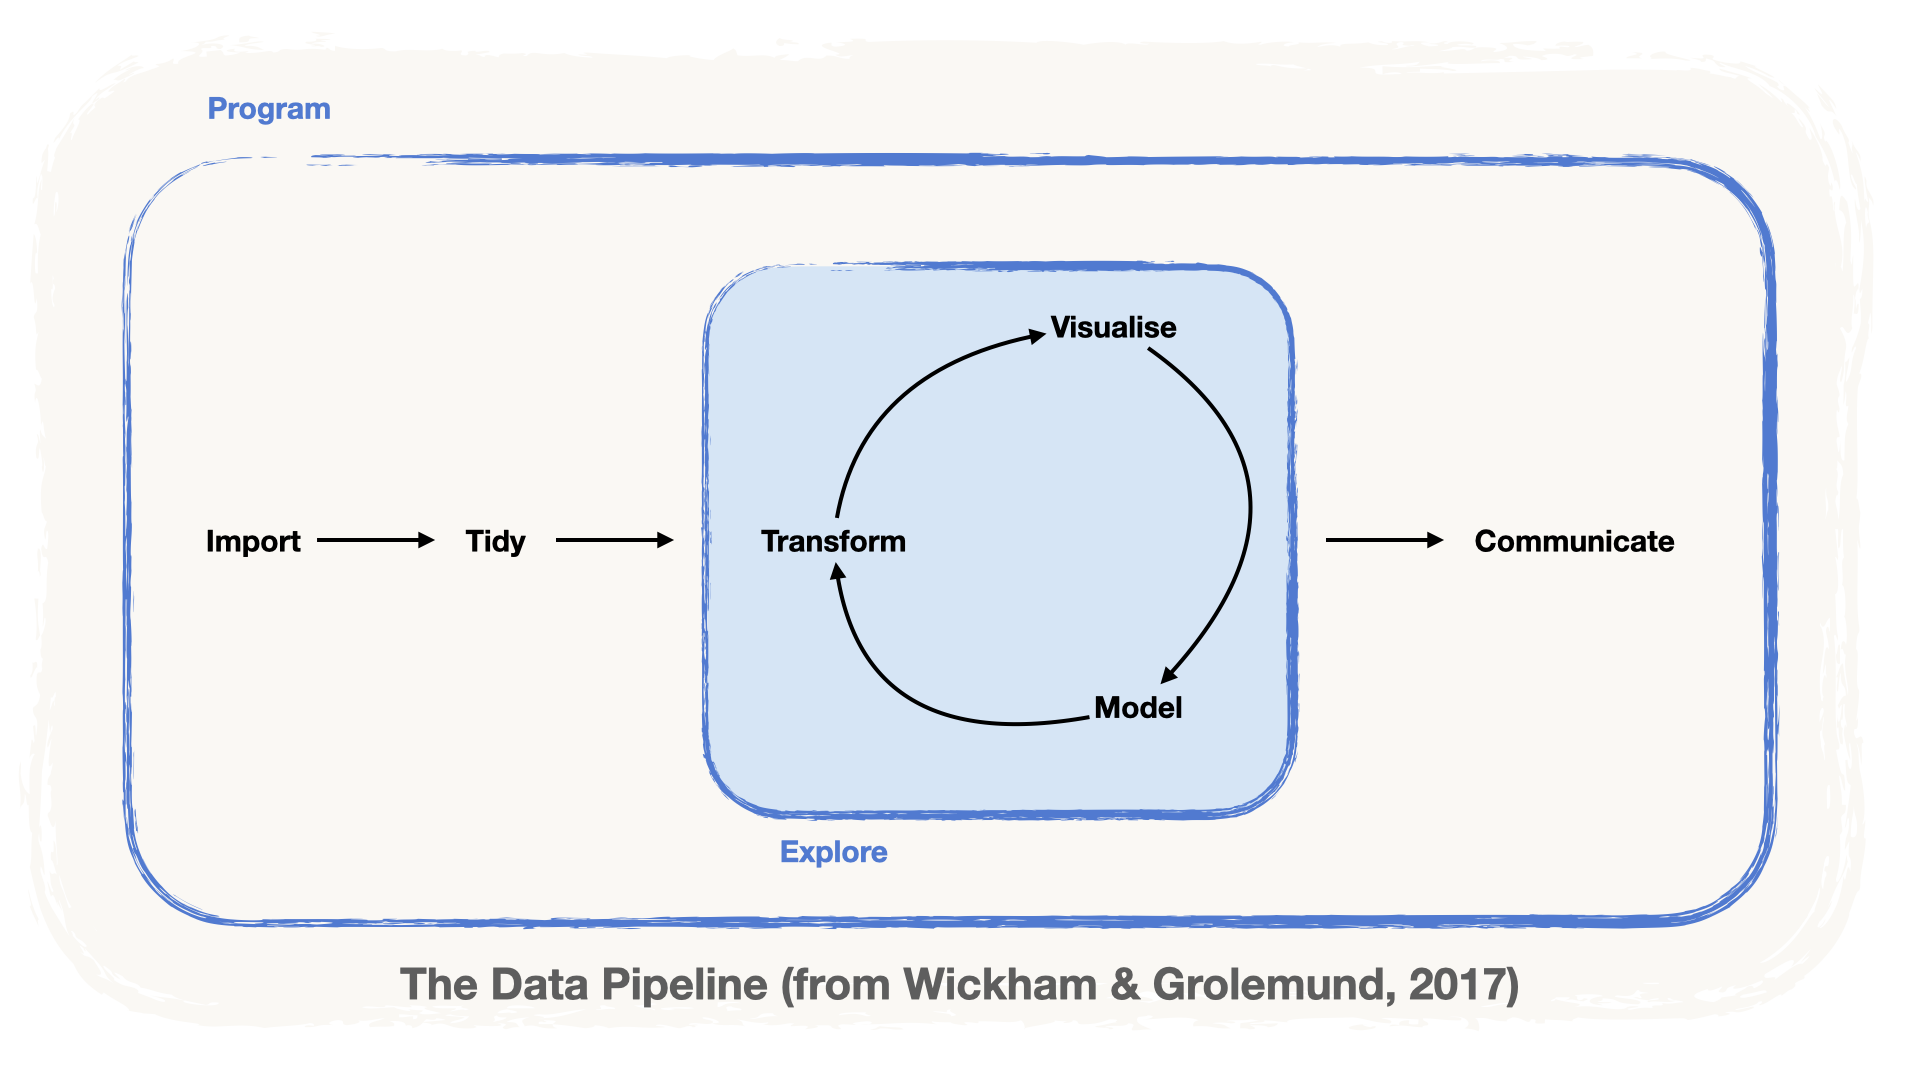
\includegraphics{img/fig-data-pipeline-empty.png}

To illustrate, we will study the stocks of \textbf{five tech companies}

\begin{itemize}
\item
  First we'll focus on a single company
\item
  Then we'll see how all these companies have fared over time.
\end{itemize}

Importing the data

\begin{itemize}
\tightlist
\item
  We've imported the data using the package \texttt{\{tidyquant\}}.
\end{itemize}

\begin{itemize}
\tightlist
\item
  The dataset contains the information on stocks for 6 companies: Apple
  Inc.~\textbf{(AAPL)}, Microsoft Corporation \textbf{(MSFT)} , Alphabet
  Inc.~\textbf{(GOOG)}, Amazon Inc.~\textbf{(AMZN)} and Tesla
  Inc.~\textbf{(TSLA).}
\end{itemize}

\begin{longtable}[]{@{}
  >{\raggedright\arraybackslash}p{(\columnwidth - 14\tabcolsep) * \real{0.0959}}
  >{\raggedright\arraybackslash}p{(\columnwidth - 14\tabcolsep) * \real{0.1507}}
  >{\raggedleft\arraybackslash}p{(\columnwidth - 14\tabcolsep) * \real{0.1233}}
  >{\raggedleft\arraybackslash}p{(\columnwidth - 14\tabcolsep) * \real{0.1233}}
  >{\raggedleft\arraybackslash}p{(\columnwidth - 14\tabcolsep) * \real{0.1233}}
  >{\raggedleft\arraybackslash}p{(\columnwidth - 14\tabcolsep) * \real{0.1233}}
  >{\raggedleft\arraybackslash}p{(\columnwidth - 14\tabcolsep) * \real{0.1370}}
  >{\raggedleft\arraybackslash}p{(\columnwidth - 14\tabcolsep) * \real{0.1233}}@{}}

\caption{\label{tbl-data}The first six lines of the whole dataset}

\tabularnewline

\toprule\noalign{}
\begin{minipage}[b]{\linewidth}\raggedright
symbol
\end{minipage} & \begin{minipage}[b]{\linewidth}\raggedright
date
\end{minipage} & \begin{minipage}[b]{\linewidth}\raggedleft
open
\end{minipage} & \begin{minipage}[b]{\linewidth}\raggedleft
high
\end{minipage} & \begin{minipage}[b]{\linewidth}\raggedleft
low
\end{minipage} & \begin{minipage}[b]{\linewidth}\raggedleft
close
\end{minipage} & \begin{minipage}[b]{\linewidth}\raggedleft
volume
\end{minipage} & \begin{minipage}[b]{\linewidth}\raggedleft
adjusted
\end{minipage} \\
\midrule\noalign{}
\endhead
\bottomrule\noalign{}
\endlastfoot
AAPL & 2014-01-02 & 19.84571 & 19.89393 & 19.71500 & 19.75464 &
234684800 & 17.29665 \\
AAPL & 2014-01-03 & 19.74500 & 19.77500 & 19.30107 & 19.32071 &
392467600 & 16.91672 \\
AAPL & 2014-01-06 & 19.19464 & 19.52857 & 19.05714 & 19.42607 &
412610800 & 17.00897 \\
AAPL & 2014-01-07 & 19.44000 & 19.49857 & 19.21143 & 19.28714 &
317209200 & 16.88733 \\
AAPL & 2014-01-08 & 19.24321 & 19.48429 & 19.23893 & 19.40929 &
258529600 & 16.99427 \\
AAPL & 2014-01-09 & 19.52857 & 19.53071 & 19.11964 & 19.16143 &
279148800 & 16.77725 \\

\end{longtable}

Tidying the data

\section{Choosing a Company}

\begin{itemize}
\item
  A ticker can be stored in the variable \texttt{company\_ticker}.
\item
  Later, this will help us \emph{parametrise} our report
\end{itemize}

\section{Choosing a Timeframe}

\begin{itemize}
\item
  To narrow our focus, we restrain our analysis to a given timeframe.
\item
  We will focus on the performance of these stocks since the beginning
  of the COVID-19 pandemic (March 11 2020) until now.
\item
  The \texttt{start\_date} variable can store this information.
\end{itemize}

\section{Filtering the data}

\begin{itemize}
\item
  We're interested in the company APPLE INC, we can use the ticker AAPL
\item
  We'll use the \texttt{filter()} to subset the data for the company in
  the given timeframe.
\end{itemize}

\begin{itemize}
\tightlist
\item
  We can explore the data by printing its first 6 lines:
\end{itemize}

\begin{longtable}[]{@{}
  >{\raggedright\arraybackslash}p{(\columnwidth - 14\tabcolsep) * \real{0.1014}}
  >{\raggedright\arraybackslash}p{(\columnwidth - 14\tabcolsep) * \real{0.1594}}
  >{\raggedleft\arraybackslash}p{(\columnwidth - 14\tabcolsep) * \real{0.1159}}
  >{\raggedleft\arraybackslash}p{(\columnwidth - 14\tabcolsep) * \real{0.1159}}
  >{\raggedleft\arraybackslash}p{(\columnwidth - 14\tabcolsep) * \real{0.1159}}
  >{\raggedleft\arraybackslash}p{(\columnwidth - 14\tabcolsep) * \real{0.1159}}
  >{\raggedleft\arraybackslash}p{(\columnwidth - 14\tabcolsep) * \real{0.1449}}
  >{\raggedleft\arraybackslash}p{(\columnwidth - 14\tabcolsep) * \real{0.1304}}@{}}

\caption{\label{tbl-clean-data}The first six lines of the apple dataset}

\tabularnewline

\toprule\noalign{}
\begin{minipage}[b]{\linewidth}\raggedright
symbol
\end{minipage} & \begin{minipage}[b]{\linewidth}\raggedright
date
\end{minipage} & \begin{minipage}[b]{\linewidth}\raggedleft
open
\end{minipage} & \begin{minipage}[b]{\linewidth}\raggedleft
high
\end{minipage} & \begin{minipage}[b]{\linewidth}\raggedleft
low
\end{minipage} & \begin{minipage}[b]{\linewidth}\raggedleft
close
\end{minipage} & \begin{minipage}[b]{\linewidth}\raggedleft
volume
\end{minipage} & \begin{minipage}[b]{\linewidth}\raggedleft
adjusted
\end{minipage} \\
\midrule\noalign{}
\endhead
\bottomrule\noalign{}
\endlastfoot
AAPL & 2020-03-12 & 63.9850 & 67.5000 & 62.0000 & 62.0575 & 418474000 &
60.52466 \\
AAPL & 2020-03-13 & 66.2225 & 69.9800 & 63.2375 & 69.4925 & 370732000 &
67.77602 \\
AAPL & 2020-03-16 & 60.4875 & 64.7700 & 60.0000 & 60.5525 & 322423600 &
59.05683 \\
AAPL & 2020-03-17 & 61.8775 & 64.4025 & 59.6000 & 63.2150 & 324056000 &
61.65356 \\
AAPL & 2020-03-18 & 59.9425 & 62.5000 & 59.2800 & 61.6675 & 300233600 &
60.14429 \\
AAPL & 2020-03-19 & 61.8475 & 63.2100 & 60.6525 & 61.1950 & 271857200 &
59.68346 \\

\end{longtable}

Understanding the data

\section{Visualise}\label{visualise}

\begin{itemize}
\item
  With this data and the functions in \texttt{ggplot()}, we can create a
  first visualisation of the closing stock price (\texttt{close}).
\item
  We set the dates on the \texttt{x} axis and the \texttt{close} price
  in the \texttt{y} axis.
\end{itemize}

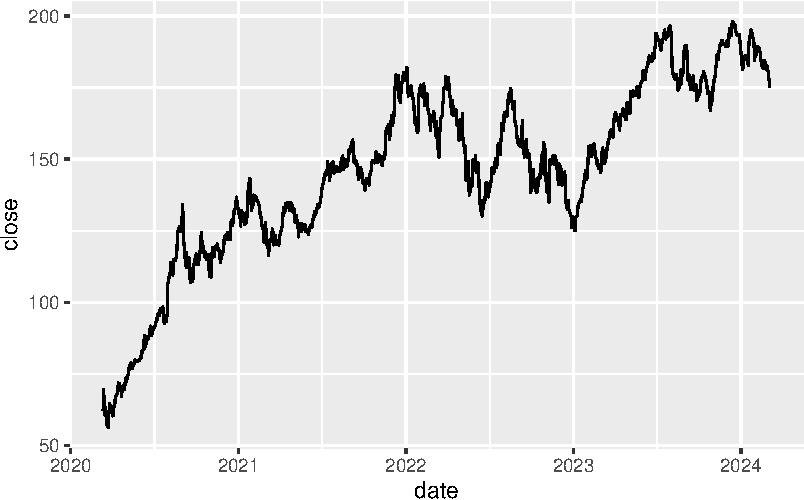
\includegraphics{jasa_files/figure-pdf/unnamed-chunk-6-1.pdf}

\section{Transform}\label{transform}

\begin{itemize}
\item
  The visualisation offers a first glance. We can transform again to ask
  the questions on the returns.
\item
  Remember that the difference in log-price are approximations of the
  returns, i.e.~the \textbf{percentage gain after selling the stock}.
\end{itemize}

\begin{definition}[]\protect\hypertarget{def-log-returns}{}\label{def-log-returns}

Let \(p_t\) denote the closing price of the stock, the log-return
\(r_t\) can be defined as:
\begin{equation}\phantomsection\label{eq-return-definition}{
r_t = \log(p_t) - \log(p_{t-1}) \approx \frac{p_t - p_{t-1}}{p_{t-1}}
}\end{equation}

\end{definition}

\begin{itemize}
\tightlist
\item
  We use the function \texttt{mutate()}, alongside \texttt{lag()} to
  create a column with the daily (log) returns and the definition in
  equation Definition~\ref{def-log-returns}
\end{itemize}

\section{Visualize again:
log-returns}\label{visualize-again-log-returns}

We can construct a visualisation with this. Additionally, we can add
layers to our visualisation to decorate it at will.

\begin{figure}

\centering{

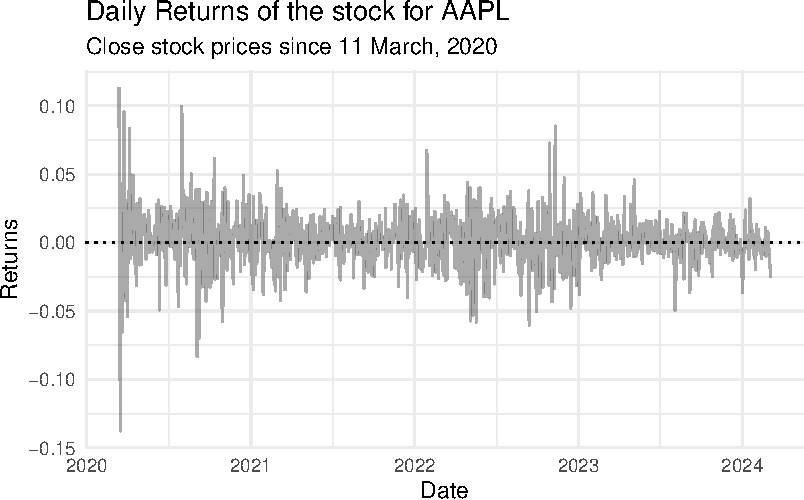
\includegraphics{jasa_files/figure-pdf/fig-log-returns-aapl-1.pdf}

}

\caption{\label{fig-log-returns-aapl}Log-returns for AAPL}

\end{figure}%

\begin{tcolorbox}[enhanced jigsaw, titlerule=0mm, toptitle=1mm, bottomrule=.15mm, left=2mm, arc=.35mm, colframe=quarto-callout-important-color-frame, rightrule=.15mm, opacityback=0, coltitle=black, colbacktitle=quarto-callout-important-color!10!white, title=\textcolor{quarto-callout-important-color}{\faExclamation}\hspace{0.5em}{Look at the years!}, bottomtitle=1mm, breakable, leftrule=.75mm, colback=white, opacitybacktitle=0.6, toprule=.15mm]

What can you say about this plot?

\begin{itemize}
\item
  It appears that there is a high \textbf{variability} of the
  log-returns in the year 2020
\item
  This increase in \textbf{variance} seems to stabilise in 2021 and
  \textbf{reappear} in 2022
\item
  The year 2023 is also quite stable
\end{itemize}

All these point to signs of increased \textbf{variability} in times of
\textbf{global crises}, which have added elements of uncertainty to the
global supply chain.

\end{tcolorbox}

\section{Model: Create summary
statistics}\label{model-create-summary-statistics}

\begin{itemize}
\item
  We can obtain a summary table for some summary statistics with
  \texttt{summarise()}.
\item
  We will compute the average return \(\bar{r}\) and estimate the
  standard deviation (SD) of the log-returns \(\hat{\sigma}\)
\end{itemize}

\begin{definition}[]\protect\hypertarget{def-summary-statistics}{}\label{def-summary-statistics}

These statistics are defined as follows:

\begin{align}
  \bar{r} &= \frac{1}{T}\sum_{t=1}^T r_t\\
  \hat{\sigma}  &= \sqrt{\frac{1}{T-1}\sum_{t=1}^T \left(r_t - \bar{r}\right)^2}
\end{align}

\end{definition}

\begin{tcolorbox}[enhanced jigsaw, titlerule=0mm, toptitle=1mm, bottomrule=.15mm, left=2mm, arc=.35mm, colframe=quarto-callout-caution-color-frame, rightrule=.15mm, opacityback=0, coltitle=black, colbacktitle=quarto-callout-caution-color!10!white, title=\textcolor{quarto-callout-caution-color}{\faFire}\hspace{0.5em}{A word of warning}, bottomtitle=1mm, breakable, leftrule=.75mm, colback=white, opacitybacktitle=0.6, toprule=.15mm]

While the average return might not mean much in theoretical terms, the
standard deviation might give some idea of the \emph{risk} or
\emph{volatility}.

\end{tcolorbox}

\begin{itemize}
\tightlist
\item
  We can show the values in the following table:
\end{itemize}

\begin{longtable}{rr}

\caption{\label{tbl-summary-aapl}Summary statistics of the log-returns
for AAPL}

\tabularnewline

\caption*{
{\large Summary statistics of Tech companies stocks} \\
{\small From 11 Mar, 2020 to 05 Mar, 2024}
} \\
\toprule
Average Return & Average Risk (SD) \\
\midrule\addlinespace[2.5pt]
$0.0010$ & $0.0200$ \\
\bottomrule

\end{longtable}

\subsection{Summary statistics by
year}\label{summary-statistics-by-year}

And, seeing that the visualisation shows periods of high volatility in
the year 2020, we can compute yearly measures of risk and volatility:

\begin{longtable*}{rrr}
\caption*{
{\large Summary statistics of Tech companies stocks} \\
{\small From 11 Mar, 2020 to 05 Mar, 2024}
} \\
\toprule
year & Average Return & Risk (SD) \\
\midrule\addlinespace[2.5pt]
2020 & \cellcolor[HTML]{90EE90}{\textcolor[HTML]{FFFFFF}{$0.0037$}} & \cellcolor[HTML]{FF0000}{\textcolor[HTML]{FFFFFF}{$0.0283$}} \\
2021 & \cellcolor[HTML]{90EE90}{\textcolor[HTML]{FFFFFF}{$0.0012$}} & $0.0158$ \\
2022 & $-0.0012$ & \cellcolor[HTML]{FF0000}{\textcolor[HTML]{FFFFFF}{$0.0224$}} \\
2023 & \cellcolor[HTML]{90EE90}{\textcolor[HTML]{FFFFFF}{$0.0016$}} & $0.0128$ \\
2024 & $-0.0022$ & $0.0123$ \\
\bottomrule
\end{longtable*}

\begin{tcolorbox}[enhanced jigsaw, titlerule=0mm, toptitle=1mm, bottomrule=.15mm, left=2mm, arc=.35mm, colframe=quarto-callout-important-color-frame, rightrule=.15mm, opacityback=0, coltitle=black, colbacktitle=quarto-callout-important-color!10!white, title=\textcolor{quarto-callout-important-color}{\faExclamation}\hspace{0.5em}{Look at the years (again)!}, bottomtitle=1mm, breakable, leftrule=.75mm, colback=white, opacitybacktitle=0.6, toprule=.15mm]

We're highlighting the years where the risk is higher. These numbers
reflect the remarks we've made in the previous points, namely that
global uncertainties have affected the risk of this stock.

\end{tcolorbox}

Analyzing multiple companies

\begin{itemize}
\item
  Now we'll carry the same analysis for multiple companies
\item
  We import the data and prepare it for analysis
\end{itemize}

\section{Plotting the stock price}\label{plotting-the-stock-price}

\begin{itemize}
\tightlist
\item
  Let's plot the whole
\end{itemize}

\begin{figure}

\centering{

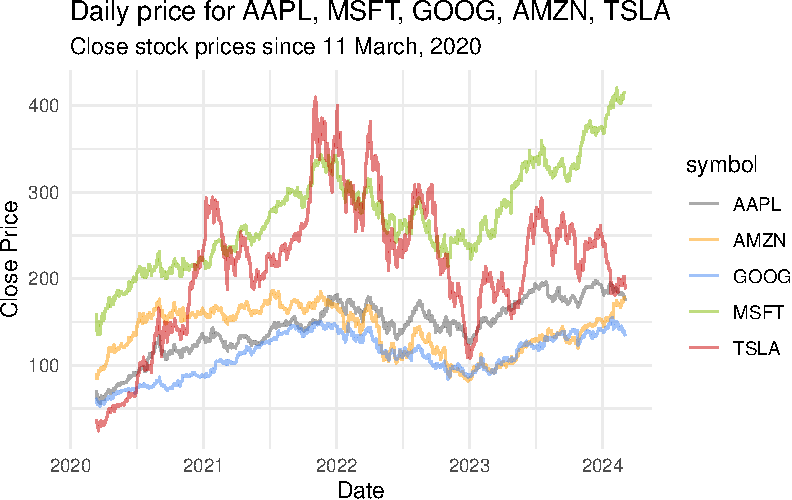
\includegraphics{jasa_files/figure-pdf/fig-all-stocks-1.pdf}

}

\caption{\label{fig-all-stocks}Stocks prices for all companies in the
selected period}

\end{figure}%

\begin{itemize}
\tightlist
\item
  A single chart is not very satisfactory, even if we try to make
  differentiate companies with colors.
\end{itemize}

\section{Visualising the log-returns}\label{visualising-the-log-returns}

\begin{itemize}
\tightlist
\item
  As the interest is in the \texttt{log}-returns, let's plot the returns
  in a single frame
\end{itemize}

\begin{figure}

\centering{

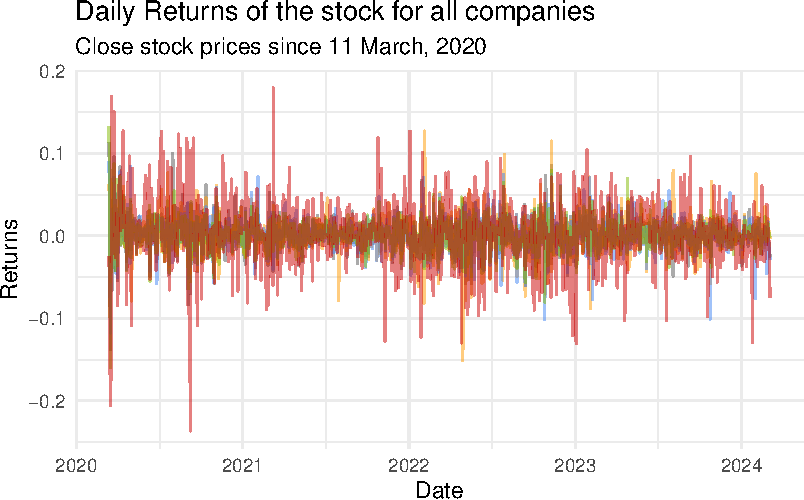
\includegraphics{jasa_files/figure-pdf/fig-log-returns-all-stocks-1.pdf}

}

\caption{\label{fig-log-returns-all-stocks}Log returns of all companies}

\end{figure}%

\begin{tcolorbox}[enhanced jigsaw, titlerule=0mm, toptitle=1mm, bottomrule=.15mm, left=2mm, arc=.35mm, colframe=quarto-callout-important-color-frame, rightrule=.15mm, opacityback=0, coltitle=black, colbacktitle=quarto-callout-important-color!10!white, title=\textcolor{quarto-callout-important-color}{\faExclamation}\hspace{0.5em}{Create a faceted chart}, bottomtitle=1mm, breakable, leftrule=.75mm, colback=white, opacitybacktitle=0.6, toprule=.15mm]

\begin{itemize}
\tightlist
\item
  There's a problem here, as you can see. The log-returns are confounded
  and become difficult to distinguish in spite of the use of relevant
  colors!
\end{itemize}

\end{tcolorbox}

\section{Creating a faceted chart}\label{creating-a-faceted-chart}

\begin{itemize}
\item
  To distinguish better, we can use the function \texttt{facet\_wrap()}
  .
\item
  This creates a \_mini\_ plot according to a variable
\end{itemize}

\begin{figure}

\centering{

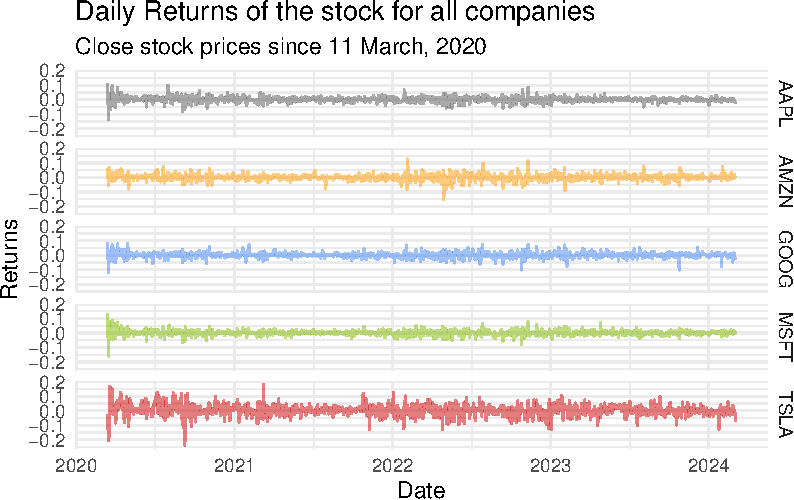
\includegraphics{jasa_files/figure-pdf/fig-log-returns-all-stocks-faceted-1.pdf}

}

\caption{\label{fig-log-returns-all-stocks-faceted}Log returns of all
companies - faceted}

\end{figure}%

\begin{enumerate}
\def\labelenumi{\arabic{enumi}.}
\tightlist
\item
  On this line we added the faceted chart
\end{enumerate}

\begin{tcolorbox}[enhanced jigsaw, titlerule=0mm, toptitle=1mm, bottomrule=.15mm, left=2mm, arc=.35mm, colframe=quarto-callout-important-color-frame, rightrule=.15mm, opacityback=0, coltitle=black, colbacktitle=quarto-callout-important-color!10!white, title=\textcolor{quarto-callout-important-color}{\faExclamation}\hspace{0.5em}{What can we see?}, bottomtitle=1mm, breakable, leftrule=.75mm, colback=white, opacitybacktitle=0.6, toprule=.15mm]

\begin{itemize}
\item
  Uncertainties in the supply chains produced by the international
  crises seem to have affected companies in the same way
\item
  However the magnitude of these impacts seems to have been different
  across companies, e.g.

  \begin{itemize}
  \tightlist
  \item
    TSLA shows significantly more risk
  \end{itemize}
\end{itemize}

\end{tcolorbox}

\section{Average Returns for all
companies}\label{average-returns-for-all-companies}

\begin{longtable}{lrrrrr}

\caption{\label{tbl-average-returns-all-companies}Average Returns for
all companies}

\tabularnewline

\caption*{
{\large Average Yearly returns of Tech companies} \\
{\small From 11 Mar, 2020 to 05 Mar, 2024}
} \\
\toprule
symbol & 2020 & 2021 & 2022 & 2023 & 2024 \\
\midrule\addlinespace[2.5pt]
AAPL & \cellcolor[HTML]{90EE90}{\textcolor[HTML]{FFFFFF}{$0.0037$}} & \cellcolor[HTML]{90EE90}{\textcolor[HTML]{FFFFFF}{$0.0012$}} & \cellcolor[HTML]{FF0000}{\textcolor[HTML]{FFFFFF}{$-0.0012$}} & \cellcolor[HTML]{90EE90}{\textcolor[HTML]{FFFFFF}{$0.0016$}} & \cellcolor[HTML]{FF0000}{\textcolor[HTML]{FFFFFF}{$-0.0022$}} \\
AMZN & \cellcolor[HTML]{90EE90}{\textcolor[HTML]{FFFFFF}{$0.0033$}} & \cellcolor[HTML]{90EE90}{\textcolor[HTML]{FFFFFF}{$0.0001$}} & \cellcolor[HTML]{FF0000}{\textcolor[HTML]{FFFFFF}{$-0.0027$}} & \cellcolor[HTML]{90EE90}{\textcolor[HTML]{FFFFFF}{$0.0024$}} & \cellcolor[HTML]{90EE90}{\textcolor[HTML]{FFFFFF}{$0.0036$}} \\
GOOG & \cellcolor[HTML]{90EE90}{\textcolor[HTML]{FFFFFF}{$0.0022$}} & \cellcolor[HTML]{90EE90}{\textcolor[HTML]{FFFFFF}{$0.0020$}} & \cellcolor[HTML]{FF0000}{\textcolor[HTML]{FFFFFF}{$-0.0019$}} & \cellcolor[HTML]{90EE90}{\textcolor[HTML]{FFFFFF}{$0.0019$}} & \cellcolor[HTML]{FF0000}{\textcolor[HTML]{FFFFFF}{$-0.0011$}} \\
MSFT & \cellcolor[HTML]{90EE90}{\textcolor[HTML]{FFFFFF}{$0.0023$}} & \cellcolor[HTML]{90EE90}{\textcolor[HTML]{FFFFFF}{$0.0016$}} & \cellcolor[HTML]{FF0000}{\textcolor[HTML]{FFFFFF}{$-0.0013$}} & \cellcolor[HTML]{90EE90}{\textcolor[HTML]{FFFFFF}{$0.0018$}} & \cellcolor[HTML]{90EE90}{\textcolor[HTML]{FFFFFF}{$0.0023$}} \\
TSLA & \cellcolor[HTML]{90EE90}{\textcolor[HTML]{FFFFFF}{$0.0090$}} & \cellcolor[HTML]{90EE90}{\textcolor[HTML]{FFFFFF}{$0.0016$}} & \cellcolor[HTML]{FF0000}{\textcolor[HTML]{FFFFFF}{$-0.0042$}} & \cellcolor[HTML]{90EE90}{\textcolor[HTML]{FFFFFF}{$0.0028$}} & \cellcolor[HTML]{FF0000}{\textcolor[HTML]{FFFFFF}{$-0.0065$}} \\
\bottomrule

\end{longtable}

\section{Risk (SD) all companies}\label{risk-sd-all-companies}

\begin{longtable}{lrrrrr}

\caption{\label{tbl-risk-all-companies}Risk (SD) all companies in the
period}

\tabularnewline

\caption*{
{\large Average Yearly SDs of Tech companies} \\
{\small From 11 Mar, 2020 to 05 Mar, 2024}
} \\
\toprule
symbol & 2020 & 2021 & 2022 & 2023 & 2024 \\
\midrule\addlinespace[2.5pt]
AAPL & \cellcolor[HTML]{FF0000}{\textcolor[HTML]{FFFFFF}{$0.0283$}} & $0.0158$ & \cellcolor[HTML]{FF0000}{\textcolor[HTML]{FFFFFF}{$0.0224$}} & $0.0128$ & $0.0123$ \\
AMZN & \cellcolor[HTML]{FF0000}{\textcolor[HTML]{FFFFFF}{$0.0237$}} & $0.0152$ & \cellcolor[HTML]{FF0000}{\textcolor[HTML]{FFFFFF}{$0.0316$}} & \cellcolor[HTML]{FF0000}{\textcolor[HTML]{FFFFFF}{$0.0207$}} & $0.0180$ \\
GOOG & \cellcolor[HTML]{FF0000}{\textcolor[HTML]{FFFFFF}{$0.0234$}} & $0.0149$ & \cellcolor[HTML]{FF0000}{\textcolor[HTML]{FFFFFF}{$0.0244$}} & $0.0193$ & $0.0185$ \\
MSFT & \cellcolor[HTML]{FF0000}{\textcolor[HTML]{FFFFFF}{$0.0268$}} & $0.0132$ & \cellcolor[HTML]{FF0000}{\textcolor[HTML]{FFFFFF}{$0.0223$}} & $0.0157$ & $0.0113$ \\
TSLA & \cellcolor[HTML]{FF0000}{\textcolor[HTML]{FFFFFF}{$0.0538$}} & \cellcolor[HTML]{FF0000}{\textcolor[HTML]{FFFFFF}{$0.0342$}} & \cellcolor[HTML]{FF0000}{\textcolor[HTML]{FFFFFF}{$0.0423$}} & \cellcolor[HTML]{FF0000}{\textcolor[HTML]{FFFFFF}{$0.0340$}} & \cellcolor[HTML]{FF0000}{\textcolor[HTML]{FFFFFF}{$0.0309$}} \\
\bottomrule

\end{longtable}


  \bibliography{bibliography.bib}


\end{document}
